\section{Introduction}
\begin{frame}{Introduction to Linear Cryptanalysis}
	\begin{columns}[T]
		\begin{column}{.58\textwidth}
			\begin{itemize}
				\item invented by Matsui 1993--1994
				\item broke DES
				\item together with Differential Cryptanalysis
						most used attack on block ciphers
			\end{itemize}
		\end{column}
		\hfill
		\begin{column}{.38\textwidth}
			\begin{figure}[!ht]
				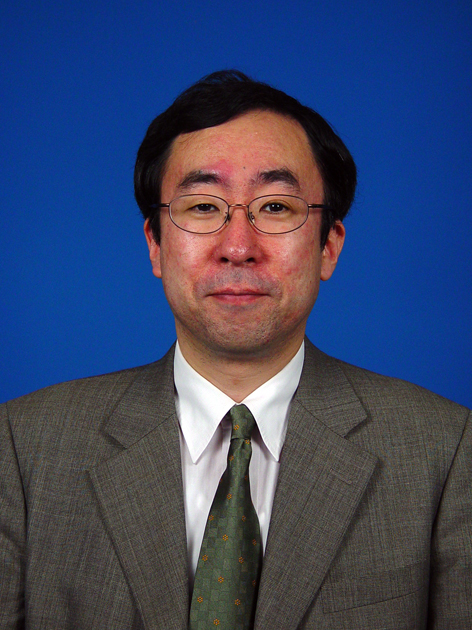
\includegraphics[height=50mm]{data/matsui.jpg}
			\end{figure}
		\end{column}
	\end{columns}\blfootnote{\scriptsize Image: \url{http://www.isce2009.ryukoku.ac.jp/eng/keynote_address.html}}
\end{frame}

\section{\present{} \& Linear Cryptanalysis}
\begin{frame}{\present{}}
	\begin{figure}[!ht]
		\centering
		\begin{tikzpicture}[%
				x={(0.04\textwidth,0)},
				y={(0,0.03\textwidth)},
				spy using outlines={%
					saphierblau,
					circle,
					magnification=13,
					size=200,
					connect spies
				}
			]

			\def \maxround{2}
			\def \roundH{5}
			\def \round{1}

			\def \TEST{\roundH*\maxround-\roundH*\round+0.5}
			\def \BEST{\roundH*\maxround-\roundH*\round-\roundH+2.5}
			%Sboxes with input and output lines and xor for the key
			\foreach \i in {0,1,2,3,4,5,6,7,8,9,10,11,12,13,14,15}{%
				%Input and output lines
				\foreach \j in {1,2,3,4}{%
					%output lines
					\draw[color=saphierblau] (1.5*\i+0.2*\j,\roundH*\maxround-\roundH*\round+1) -- (1.5*\i+0.2*\j,\roundH*\maxround-\roundH*\round+0.5);

					%input lines
					\draw[color=saphierblau] (1.5*\i+0.2*\j,\roundH*\maxround-\roundH*\round+2) -- (1.5*\i+0.2*\j,\roundH*\maxround-\roundH*\round+2.5);

					%XOR
					\draw[color=saphierblau] (1.5*\i+0.2*\j,\roundH*\maxround-\roundH*\round+2.25) circle (0.1);
					\draw[color=saphierblau] (1.5*\i+0.2*\j-0.1,\roundH*\maxround-\roundH*\round+2.25) -- (1.5*\i+0.2*\j+0.1,\roundH*\maxround-\roundH*\round+2.25);
				}

				%Sbox
				\draw[color=black] (1.5*\i,\roundH*\maxround-\roundH*\round+1) rectangle (1.5*\i+1,\roundH*\maxround-\roundH*\round+2);
				\node[color=saphierblau] at (1.5*\i+0.5,\roundH*\maxround-\roundH*\round+1.5) {S};
			}

			%The P-layer
			\draw[color=saphierblau] ( 0.2,\TEST) -- ( 0.2,\BEST); \draw[color=saphierblau] ( 0.4,\TEST) -- ( 6.2,\BEST);
			\draw[color=saphierblau] ( 0.6,\TEST) -- (12.2,\BEST); \draw[color=saphierblau] ( 0.8,\TEST) -- (18.2,\BEST);
			\draw[color=saphierblau] ( 1.7,\TEST) -- ( 0.4,\BEST); \draw[color=saphierblau] ( 1.9,\TEST) -- ( 6.4,\BEST);
			\draw[color=saphierblau] ( 2.1,\TEST) -- (12.4,\BEST); \draw[color=saphierblau] ( 2.3,\TEST) -- (18.4,\BEST);
			\draw[color=saphierblau] ( 3.2,\TEST) -- ( 0.6,\BEST); \draw[color=saphierblau] ( 3.4,\TEST) -- ( 6.6,\BEST);
			\draw[color=saphierblau] ( 3.6,\TEST) -- (12.6,\BEST); \draw[color=saphierblau] ( 3.8,\TEST) -- (18.6,\BEST);
			\draw[color=saphierblau] ( 4.7,\TEST) -- ( 0.8,\BEST); \draw[color=saphierblau] ( 4.9,\TEST) -- ( 6.8,\BEST);
			\draw[color=saphierblau] ( 5.1,\TEST) -- (12.8,\BEST); \draw[color=saphierblau] ( 5.3,\TEST) -- (18.8,\BEST);
			\draw[color=saphierblau] ( 6.2,\TEST) -- ( 1.7,\BEST); \draw[color=saphierblau] ( 6.4,\TEST) -- ( 7.7,\BEST);
			\draw[color=saphierblau] ( 6.6,\TEST) -- (13.7,\BEST); \draw[color=saphierblau] ( 6.8,\TEST) -- (19.7,\BEST);
			\draw[color=saphierblau] ( 7.7,\TEST) -- ( 1.9,\BEST); \draw[color=saphierblau] ( 7.9,\TEST) -- ( 7.9,\BEST);
			\draw[color=saphierblau] ( 8.1,\TEST) -- (13.9,\BEST); \draw[color=saphierblau] ( 8.3,\TEST) -- (19.9,\BEST);
			\draw[color=saphierblau] ( 9.2,\TEST) -- ( 2.1,\BEST); \draw[color=saphierblau] ( 9.4,\TEST) -- ( 8.1,\BEST);
			\draw[color=saphierblau] ( 9.6,\TEST) -- (14.1,\BEST); \draw[color=saphierblau] ( 9.8,\TEST) -- (20.1,\BEST);
			\draw[color=saphierblau] (10.7,\TEST) -- ( 2.3,\BEST); \draw[color=saphierblau] (10.9,\TEST) -- ( 8.3,\BEST);
			\draw[color=saphierblau] (11.1,\TEST) -- (14.3,\BEST); \draw[color=saphierblau] (11.3,\TEST) -- (20.3,\BEST);
			\draw[color=saphierblau] (12.2,\TEST) -- ( 3.2,\BEST); \draw[color=saphierblau] (12.4,\TEST) -- ( 9.2,\BEST);
			\draw[color=saphierblau] (12.6,\TEST) -- (15.2,\BEST); \draw[color=saphierblau] (12.8,\TEST) -- (21.2,\BEST);
			\draw[color=saphierblau] (13.7,\TEST) -- ( 3.4,\BEST); \draw[color=saphierblau] (13.9,\TEST) -- ( 9.4,\BEST);
			\draw[color=saphierblau] (14.1,\TEST) -- (15.4,\BEST); \draw[color=saphierblau] (14.3,\TEST) -- (21.4,\BEST);
			\draw[color=saphierblau] (15.2,\TEST) -- ( 3.6,\BEST); \draw[color=saphierblau] (15.4,\TEST) -- ( 9.6,\BEST);
			\draw[color=saphierblau] (15.6,\TEST) -- (15.6,\BEST); \draw[color=saphierblau] (15.8,\TEST) -- (21.6,\BEST);
			\draw[color=saphierblau] (16.7,\TEST) -- ( 3.8,\BEST); \draw[color=saphierblau] (16.9,\TEST) -- ( 9.8,\BEST);
			\draw[color=saphierblau] (17.1,\TEST) -- (15.8,\BEST); \draw[color=saphierblau] (17.3,\TEST) -- (21.8,\BEST);
			\draw[color=saphierblau] (18.2,\TEST) -- ( 4.7,\BEST); \draw[color=saphierblau] (18.4,\TEST) -- (10.7,\BEST);
			\draw[color=saphierblau] (18.6,\TEST) -- (16.7,\BEST); \draw[color=saphierblau] (18.8,\TEST) -- (22.7,\BEST);
			\draw[color=saphierblau] (19.7,\TEST) -- ( 4.9,\BEST); \draw[color=saphierblau] (19.9,\TEST) -- (10.9,\BEST);
			\draw[color=saphierblau] (20.1,\TEST) -- (16.9,\BEST); \draw[color=saphierblau] (20.3,\TEST) -- (22.9,\BEST);
			\draw[color=saphierblau] (21.2,\TEST) -- ( 5.1,\BEST); \draw[color=saphierblau] (21.4,\TEST) -- (11.1,\BEST);
			\draw[color=saphierblau] (21.6,\TEST) -- (17.1,\BEST); \draw[color=saphierblau] (21.8,\TEST) -- (23.1,\BEST);
			\draw[color=saphierblau] (22.7,\TEST) -- ( 5.3,\BEST); \draw[color=saphierblau] (22.9,\TEST) -- (11.3,\BEST);
			\draw[color=saphierblau] (23.1,\TEST) -- (17.3,\BEST); \draw[color=saphierblau] (23.3,\TEST) -- (23.3,\BEST);

%			\only<2,3>{%
%				\spy[
%					every spy on node/.append style={very thick},
%					every spy in node/.append style={very thick},
%					spy connection path={\draw[very thick] (tikzspyonnode) -- (tikzspyinnode);},
%						path picture extra={%
%							% draw stuff only in spy area:
%							\node<2>[%
%									rectangle,
%									fill=lichtgrau,
%									minimum width=6cm,
%									minimum height=4.5cm
%								]
%								(rect) at (path picture bounding box.center)
%								{%
%									\begin{tabular}{crrrr}
%										\toprule
%										$x$    & 0&1&2& 3\\
%										$S(x)$ &12&5&6&11\\
%										\midrule
%										$x$    &4&5& 6& 7\\
%										$S(x)$ &9&0&10&13\\
%										\midrule
%														& $\vdots$ & & & \\
%										\bottomrule
%									\end{tabular}
%							};
%							\node<3>[%
%									rectangle,
%									fill=lichtgrau,
%									minimum width=6cm,
%									minimum height=4.5cm
%								]
%								(rect) at (path picture bounding box.center)
%								{%
%									\tabcolsep=1mm
%									\robustify\bfseries
%									\begin{tabular}{rSSSSSSSS}
%										\toprule
%										 & 0& 1& 2& 3& 4& 5& 6& 7\\
%										0&16&  &  &  &  &  &  &  \\
%										1&  &  &  &  &  &-8&  &-8\\
%										2&  &  &\bfseries 4& 4&\bfseries -4&-4&  &  \\
%										3&  &  & 4& 4& 4&-4&-8&  \\
%										4&  &  &\bfseries -4& 4&\bfseries -4&-4&  & 8\\
%										5&  &  &-4& 4&-4& 4&  &$\ddots$ \\
%										\bottomrule
%									\end{tabular}
%							};
%						}
%					]
%					on (2,6.5) in node [overlay, fill=lichtgrau] at (11.5,1);
%			}
		\end{tikzpicture}
	\end{figure}
	%\vfill{}
	\begin{overprint}
		\onslide<1>
		\begin{itemize}
			\item Let $F_{k_i} : \mathbb{F}_2^{64} \rightarrow \mathbb{F}_2^{64}$ be the round function
				that xor's the key $k_i$ and applies the substitution and permutation layer.
		\end{itemize}
		\onslide<2>
		\begin{itemize}
			\item Let $F_{k_i} : \mathbb{F}_2^{64} \rightarrow \mathbb{F}_2^{64}$ be the round function
				that xor's the key $k_i$ and applies the substitution and permutation layer.
			\item Can we approximate this function?
		\end{itemize}
	\end{overprint}
	\vfill{}
\end{frame}

\begin{frame}{Linear Approximations}{Dot-Product, Masks and Linear Bias}
	\vspace{-10pt}
	\visible<1->{%
	\begin{itemize}
		\item We want to linear approximate a function $F : \mathbb{F}_2^n \rightarrow \mathbb{F}_2^n$
	\end{itemize}
	}

	\vspace{-10pt}
	\begin{columns}[T]
	\visible<2->{%
		\begin{column}{0.48\textwidth}
			\begin{block}{Dot-Product}
				\begin{equation*}
				\vspace{-2pt}
					\langle \alpha, x \rangle = \bigoplus_{i=0}^{n-1} \alpha_i x_i
				\end{equation*}
			\end{block}
		\end{column}
	}
	\visible<3->{%
		\begin{column}{0.48\textwidth}
			\begin{block}{Mask}
				Let $\alpha, \beta, x \in \mathbb{F}_2^n$ and
				%\vspace{-6pt}
				\begin{equation}
					\langle \alpha, x \rangle = \langle \beta, F(x) \rangle \label{equ:masks}
				\end{equation}
			\end{block}
		\end{column}
	}
	\end{columns}

	\visible<3->{%
	\begin{itemize}
		\item We say $\alpha$ is an \emph{input mask} and $\beta$ is an \emph{output mask}.
		\item Equation~\ref{equ:masks} does not hold for every input/output masks.
	\end{itemize}
	}
	\visible<4->{%
	\begin{itemize}
		\item It is \emph{biased}, i.e., $\text{Pr}[\langle \alpha, x \rangle = \langle
			\beta, F(x) \rangle] = \frac{1}{2} - \epsilon(\alpha, \beta)$.
	\end{itemize}
	}
\end{frame}

\begin{frame}{\present{}}{S-box and Linear Approximation Table}
	\vspace{-10pt}
	\begin{figure}[!ht]
		\centering
		\begin{tikzpicture}[%
				x={(0.04\textwidth,0)},
				y={(0,0.03\textwidth)},
				spy using outlines={%
					saphierblau,
					circle,
					magnification=13,
					size=200,
					connect spies
				}
			]

			\def \maxround{2}
			\def \roundH{5}
			\def \round{1}

			\def \TEST{\roundH*\maxround-\roundH*\round+0.5}
			\def \BEST{\roundH*\maxround-\roundH*\round-\roundH+2.5}
			%Sboxes with input and output lines and xor for the key
			\foreach \i in {0,1,2,3,4,5,6,7,8,9,10,11,12,13,14,15}{%
				%Input and output lines
				\foreach \j in {1,2,3,4}{%
					%output lines
					\draw[color=gray] (1.5*\i+0.2*\j,\roundH*\maxround-\roundH*\round+1) -- (1.5*\i+0.2*\j,\roundH*\maxround-\roundH*\round+0.5);

					%input lines
					\draw[color=gray] (1.5*\i+0.2*\j,\roundH*\maxround-\roundH*\round+2) -- (1.5*\i+0.2*\j,\roundH*\maxround-\roundH*\round+2.5);

					%XOR
					\draw[color=gray] (1.5*\i+0.2*\j,\roundH*\maxround-\roundH*\round+2.25) circle (0.1);
					\draw[color=gray] (1.5*\i+0.2*\j-0.1,\roundH*\maxround-\roundH*\round+2.25) -- (1.5*\i+0.2*\j+0.1,\roundH*\maxround-\roundH*\round+2.25);
				}

				%Sbox
				\draw[color=black] (1.5*\i,\roundH*\maxround-\roundH*\round+1) rectangle (1.5*\i+1,\roundH*\maxround-\roundH*\round+2);
				\node[color=saphierblau] at (1.5*\i+0.5,\roundH*\maxround-\roundH*\round+1.5) {S};
			}

			%The P-layer
			\draw[color=gray] ( 0.2,\TEST) -- ( 0.2,\BEST); \draw[color=gray] ( 0.4,\TEST) -- ( 6.2,\BEST);
			\draw[color=gray] ( 0.6,\TEST) -- (12.2,\BEST); \draw[color=gray] ( 0.8,\TEST) -- (18.2,\BEST);
			\draw[color=gray] ( 1.7,\TEST) -- ( 0.4,\BEST); \draw[color=gray] ( 1.9,\TEST) -- ( 6.4,\BEST);
			\draw[color=gray] ( 2.1,\TEST) -- (12.4,\BEST); \draw[color=gray] ( 2.3,\TEST) -- (18.4,\BEST);
			\draw[color=gray] ( 3.2,\TEST) -- ( 0.6,\BEST); \draw[color=gray] ( 3.4,\TEST) -- ( 6.6,\BEST);
			\draw[color=gray] ( 3.6,\TEST) -- (12.6,\BEST); \draw[color=gray] ( 3.8,\TEST) -- (18.6,\BEST);
			\draw[color=gray] ( 4.7,\TEST) -- ( 0.8,\BEST); \draw[color=gray] ( 4.9,\TEST) -- ( 6.8,\BEST);
			\draw[color=gray] ( 5.1,\TEST) -- (12.8,\BEST); \draw[color=gray] ( 5.3,\TEST) -- (18.8,\BEST);
			\draw[color=gray] ( 6.2,\TEST) -- ( 1.7,\BEST); \draw[color=gray] ( 6.4,\TEST) -- ( 7.7,\BEST);
			\draw[color=gray] ( 6.6,\TEST) -- (13.7,\BEST); \draw[color=gray] ( 6.8,\TEST) -- (19.7,\BEST);
			\draw[color=gray] ( 7.7,\TEST) -- ( 1.9,\BEST); \draw[color=gray] ( 7.9,\TEST) -- ( 7.9,\BEST);
			\draw[color=gray] ( 8.1,\TEST) -- (13.9,\BEST); \draw[color=gray] ( 8.3,\TEST) -- (19.9,\BEST);
			\draw[color=gray] ( 9.2,\TEST) -- ( 2.1,\BEST); \draw[color=gray] ( 9.4,\TEST) -- ( 8.1,\BEST);
			\draw[color=gray] ( 9.6,\TEST) -- (14.1,\BEST); \draw[color=gray] ( 9.8,\TEST) -- (20.1,\BEST);
			\draw[color=gray] (10.7,\TEST) -- ( 2.3,\BEST); \draw[color=gray] (10.9,\TEST) -- ( 8.3,\BEST);
			\draw[color=gray] (11.1,\TEST) -- (14.3,\BEST); \draw[color=gray] (11.3,\TEST) -- (20.3,\BEST);
			\draw[color=gray] (12.2,\TEST) -- ( 3.2,\BEST); \draw[color=gray] (12.4,\TEST) -- ( 9.2,\BEST);
			\draw[color=gray] (12.6,\TEST) -- (15.2,\BEST); \draw[color=gray] (12.8,\TEST) -- (21.2,\BEST);
			\draw[color=gray] (13.7,\TEST) -- ( 3.4,\BEST); \draw[color=gray] (13.9,\TEST) -- ( 9.4,\BEST);
			\draw[color=gray] (14.1,\TEST) -- (15.4,\BEST); \draw[color=gray] (14.3,\TEST) -- (21.4,\BEST);
			\draw[color=gray] (15.2,\TEST) -- ( 3.6,\BEST); \draw[color=gray] (15.4,\TEST) -- ( 9.6,\BEST);
			\draw[color=gray] (15.6,\TEST) -- (15.6,\BEST); \draw[color=gray] (15.8,\TEST) -- (21.6,\BEST);
			\draw[color=gray] (16.7,\TEST) -- ( 3.8,\BEST); \draw[color=gray] (16.9,\TEST) -- ( 9.8,\BEST);
			\draw[color=gray] (17.1,\TEST) -- (15.8,\BEST); \draw[color=gray] (17.3,\TEST) -- (21.8,\BEST);
			\draw[color=gray] (18.2,\TEST) -- ( 4.7,\BEST); \draw[color=gray] (18.4,\TEST) -- (10.7,\BEST);
			\draw[color=gray] (18.6,\TEST) -- (16.7,\BEST); \draw[color=gray] (18.8,\TEST) -- (22.7,\BEST);
			\draw[color=gray] (19.7,\TEST) -- ( 4.9,\BEST); \draw[color=gray] (19.9,\TEST) -- (10.9,\BEST);
			\draw[color=gray] (20.1,\TEST) -- (16.9,\BEST); \draw[color=gray] (20.3,\TEST) -- (22.9,\BEST);
			\draw[color=gray] (21.2,\TEST) -- ( 5.1,\BEST); \draw[color=gray] (21.4,\TEST) -- (11.1,\BEST);
			\draw[color=gray] (21.6,\TEST) -- (17.1,\BEST); \draw[color=gray] (21.8,\TEST) -- (23.1,\BEST);
			\draw[color=gray] (22.7,\TEST) -- ( 5.3,\BEST); \draw[color=gray] (22.9,\TEST) -- (11.3,\BEST);
			\draw[color=gray] (23.1,\TEST) -- (17.3,\BEST); \draw[color=gray] (23.3,\TEST) -- (23.3,\BEST);

			\only<2,3>{%
				\spy[
					every spy on node/.append style={very thick},
					every spy in node/.append style={very thick},
					spy connection path={\draw[very thick] (tikzspyonnode) -- (tikzspyinnode);},
						path picture extra={%
							% draw stuff only in spy area:
							\node<2>[%
									rectangle,
									fill=lichtgrau,
									minimum width=6cm,
									minimum height=4.5cm
								]
								(rect) at (path picture bounding box.center)
								{%
									\begin{tabular}{crrrr}
										\toprule
										$x$    & 0&1&2& 3\\
										$S(x)$ &12&5&6&11\\
										\midrule
										$x$    &4&5& 6& 7\\
										$S(x)$ &9&0&10&13\\
										\midrule
														& $\vdots$ & & & \\
										\bottomrule
									\end{tabular}
							};
							\node<3>[%
									rectangle,
									fill=lichtgrau,
									minimum width=6cm,
									minimum height=4.5cm
								]
								(rect) at (path picture bounding box.center)
								{%
									\tabcolsep=1mm
									\robustify\bfseries
									\begin{tabular}{rSSSSSSSS}
										\toprule
										 & 0& 1& 2& 3& 4& 5& 6& 7\\
										0&16&  &  &  &  &  &  &  \\
										1&  &  &  &  &  &-8&  &-8\\
										2&  &  &\bfseries 4& 4&\bfseries -4&-4&  &  \\
										3&  &  & 4& 4& 4&-4&-8&  \\
										4&  &  &\bfseries -4& 4&\bfseries -4&-4&  & 8\\
										5&  &  &-4& 4&-4& 4&  &$\ddots$ \\
										\bottomrule
									\end{tabular}
							};
						}
					]
					on (2,6.5) in node [overlay, fill=lichtgrau] at (11.5,1);
			}
		\end{tikzpicture}
	\end{figure}
	%\vfill{}
	\begin{overprint}
		\onslide<1>
		\begin{itemize}
			\item The only difficult part of $F_{k_i}$ is the (non-linear) substitution layer.
		\end{itemize}
		\onslide<2>
	\end{overprint}
	\vfill{}
\end{frame}

\section{Distributions}
\begin{frame}{Distributions}
	\visible<1->{%
	\begin{itemize}
		\item Attack complexity of linear cryptanalysis is proportional to $\frac{1}{\epsilon^2}$.
		\item In experiments, we observe a key dependency of the linear bias.
	\end{itemize}
	}
	\visible<2->{%
	\begin{itemize}
		\item The distribution of linear biases follows a normal distribution.
		\item Its width is defined by the variance.
	\end{itemize}
	}
	\visible<3->{%
	\begin{itemize}
		\item What happens with different key-schedules?
	\end{itemize}
	}
\end{frame}

\begin{frame}{Distributions}{Independent Round Keys}
	\begin{figure}
		\centering
		\begin{tikzpicture}
			\begin{axis}[
					every axis/.append style={font=\small},
					scaled ticks=false,
					no markers,
					xmin=-0.0002,
					ymin=0,
					ymax=475,
					xmax=0.0002,
					xlabel={Linear Correlation},
					height=7cm,
					width=11cm,
					ytick=\empty,
					xticklabels={-0.0002, -0.0001, 0, 0.0001, 0.0002},
					xtick={-0.0002, -0.0001, 0, 0.0001, 0.0002},
				]
				\addplot+[color=saphierblau, ybar, bar width=1pt, fill=saphierblau] table [x, y, col sep=space] {data/histo_indp.dat};
				\addplot+[color=red] table {data/gauss_est.dat};
				\draw[color=black, thin, dashed] (axis cs:-0.00005,\pgfkeysvalueof{/pgfplots/ymin}) -- (axis cs:-0.00005,\pgfkeysvalueof{/pgfplots/ymax});
				\draw[color=black, thin, dashed] (axis cs:0.00005,\pgfkeysvalueof{/pgfplots/ymin}) -- (axis cs:0.00005,\pgfkeysvalueof{/pgfplots/ymax});
			\end{axis}
		\end{tikzpicture}
	\end{figure}
\end{frame}

\begin{frame}{Distributions}{Constant Round Keys}
	\begin{figure}
		\centering
		\begin{tikzpicture}
			\begin{axis}[
					every axis/.append style={font=\small},
					scaled ticks=false,
					no markers,
					xmin=-0.0002,
					ymin=0,
					ymax=475,
					xmax=0.0002,
					xlabel={Linear Correlation},
					height=7cm,
					width=11cm,
					ytick=\empty,
					xticklabels={-0.0002, -0.0001, 0, 0.0001, 0.0002},
					xtick={-0.0002, -0.0001, 0, 0.0001, 0.0002},
				]
				\addplot+[color=saphierblau, ybar, bar width=1pt, fill=saphierblau] table [x, y, col sep=space] {data/histo_id.dat};
				\addplot+[color=red] table {data/gauss_est.dat};
				\draw[color=black, thin, dashed] (axis cs:-0.00005,\pgfkeysvalueof{/pgfplots/ymin}) -- (axis cs:-0.00005,\pgfkeysvalueof{/pgfplots/ymax});
				\draw[color=black, thin, dashed] (axis cs:0.00005,\pgfkeysvalueof{/pgfplots/ymin}) -- (axis cs:0.00005,\pgfkeysvalueof{/pgfplots/ymax});
			\end{axis}
		\end{tikzpicture}
	\end{figure}
\end{frame}
